
% thermal conductivity
\subsubsection{Thermal Conductivity}
G10 is an epoxy-impregnated fiberglass, thermally anisotropic. It means that its thermal conductivity along the fibers is higher than across them. In order to simplify computation in the scope of this thesis, the material is assumed to be isotropic. A conservative assumption is made which states that thermal conductivity of G10 in all directions is equal to the one normal to the direction of the fibers.
G10 thermal conductivity as well as specific heat capacity is approximated with the NIST polynomial interpolation:
\begin{equation}
    x(T) = 10^{\sum_{n=0}^{N} a_\text{n}(\log_\text{10}T)^{n}},
\end{equation}
\\
where $N$ refers to the order of polynomial and $x(T)$ is the considered material property. Fig. \ref{fig:g10_k_plot} presents G10 heat conductivity based on polynomial fit parameters depicted in Table \ref{table:nist_g10_k_parameters}.

\begin{table}[h!]
    \caption{Fit parameters for NIST G10 thermal conductivity} 
    \vspace{-1.em} 
    \fontsize{10}{10}
    \selectfont 
    \renewcommand{\arraystretch}{1.5}
    \begin{center}
    \begin{tabular}{ ccccccccc }  
    $\text{a}_0$ & $\text{a}_1$ & $\text{a}_2$ & $\text{a}_3$ & $\text{a}_4$ & $\text{a}_5$ & $\text{a}_6$ & $\text{a}_7$ & $\text{a}_8$ \\
    \hline
    -4.1236 & 13.788 & -26.068 & 26.272 & -14.663 & 4.4954 & -0.6905 & 0.0397 & 0 \\
    \hline 
    \end{tabular}
    \end{center}  
     \label{table:nist_g10_k_parameters} 
 \end{table}
 
  \begin{figure}[h!]
    \centering
    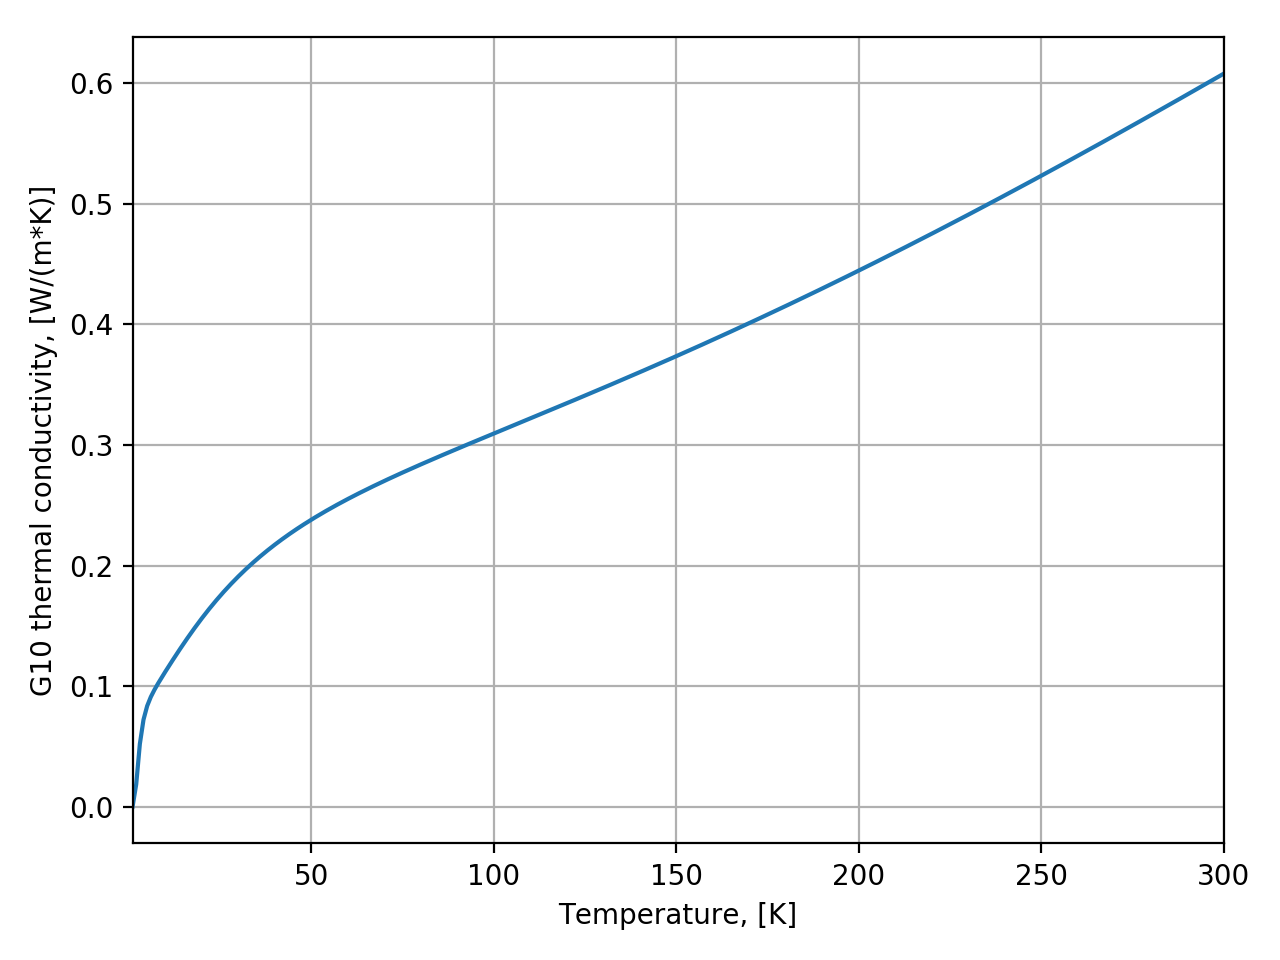
\includegraphics[width=0.49\linewidth]{figures/material_properties/G10_k_plot.png}
    \caption{G10 heat conductivity temperature dependence}
    \label{fig:g10_k_plot}
\end{figure}
 
% mass density
 \subsubsection{Mass Density}
 The mass density is assumed to be constant and equal to $\rho = 1948~\text{kg/m}^{3}$ according to NIST standards.

% specific heat capacity
\subsubsection{Specific Heat Capacity}
Fig. \ref{fig:g10_cp_plot} presents G10 specific heat capacity function based on polynomial fit parameters depicted in Table \ref{table:nist_g10_cp_parameters}.

\begin{table}[h!]
    \caption{Fit parameters for NIST G10 specific heat capacity} 
    \vspace{-1.em} 
    \fontsize{10}{10}
    \selectfont 
    \renewcommand{\arraystretch}{1.5}
    \begin{center}
    \begin{tabular}{ cccccccc }  
    $\text{a}_0$ & $\text{a}_1$ & $\text{a}_2$ & $\text{a}_3$ & $\text{a}_4$ & $\text{a}_5$ & $\text{a}_6$ & $\text{a}_7$ \\
    \hline
    -2.4083 & 7.6006 & -8.2982 & 7.3301 & -4.2386 & 1.4294 & -0.24396 & 0.015236 \\
    \hline 
    \end{tabular}
    \end{center}  
     \label{table:nist_g10_cp_parameters} 
 \end{table}

 \begin{figure}[h!]
    \centering
    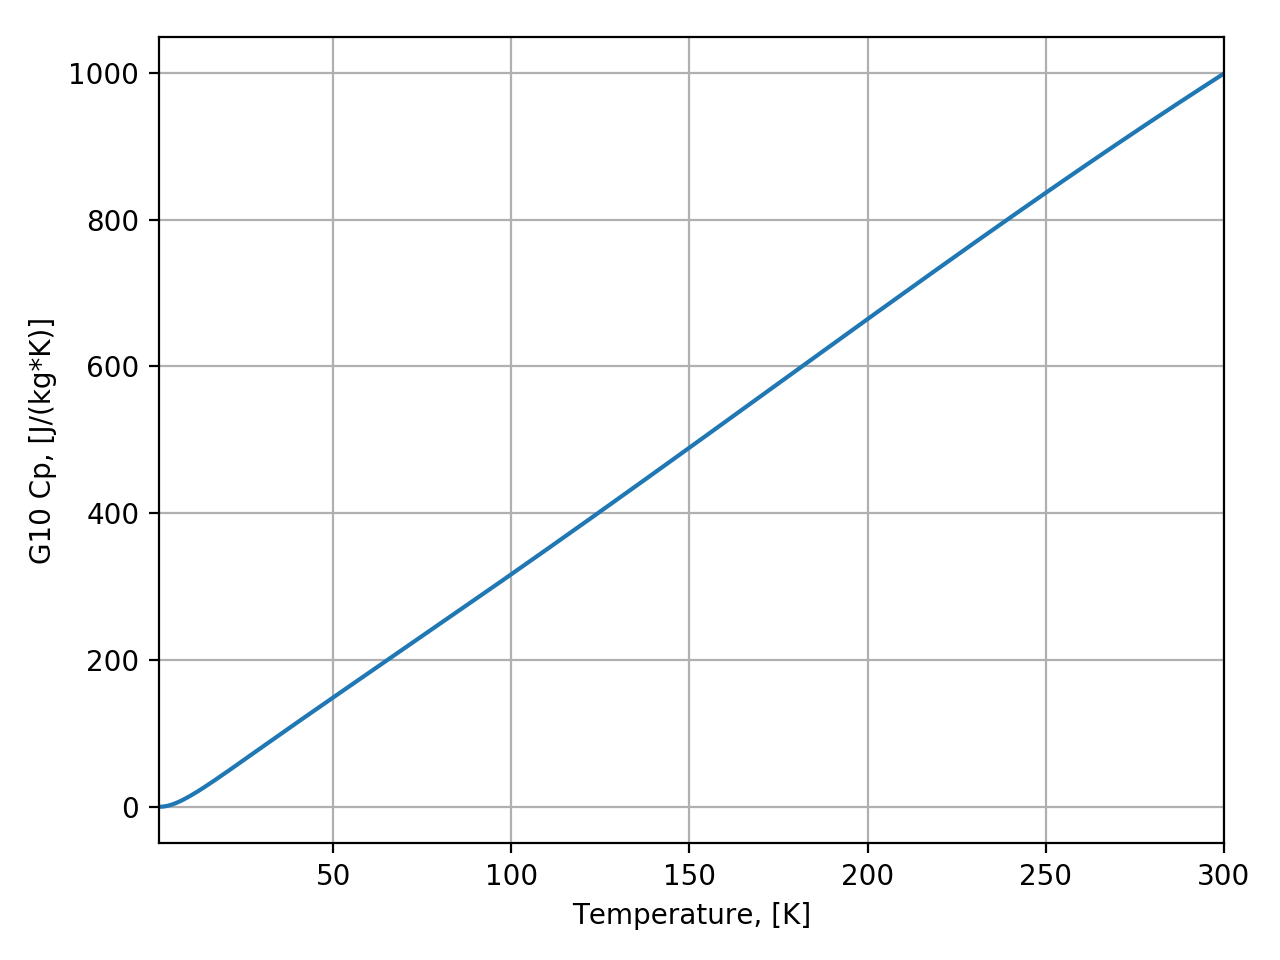
\includegraphics[width=0.49\linewidth]{figures/material_properties/G10_Cp_plot.png}
    \caption{G10 specific heat capacity temperature dependence}
    \label{fig:g10_cp_plot}
\end{figure}